\subsection{Sesto sprint}

\begin{minipage}{\textwidth}
  Di seguito è riportata la distribuzione delle ore per ciascun membro del team, accumulate in totali per persona e per ruolo:
  \begin{table}[H]
    \begin{tabularx}{\textwidth}{|c|*{6}{>{\centering}X|}c|}
      \hline
      \multicolumn{8}{|c|}{\textbf{Consuntivo orario}} \\
      \hline
      \textbf{Membro del team} & \textbf{Re} & \textbf{Am} & \textbf{An} & \textbf{Pt} & \textbf{Pr} & \textbf{Ve} & \textbf{Totale per persona} \\
      \hline
      Cavalli Riccardo & 0 & 1 & 3 & 0 & 0 & 0 & 4 \\ 
      \hline
      Pianon Raul & 0 & 3 & 1 & 0 & 0 & 0 & 4 \\ 
      \hline
      Dall’Amico Martina & 1 & 0 & 0 & 0 & 3 & 1 & 5 \\ 
      \hline
      Cristo Marco & 0 & 1 & 1 & 0 & 0 & 1 & 3 \\ 
      \hline
      Lewental Sebastiano & 3 & 0 & 0 & 0 & 1 & 0 & 4 \\ 
      \hline
      Zecchinato Mattia & 0 & 2 & 0 & 0 & 2 & 1 & 5 \\ 
      \hline
      Stocco Tommaso & 0 & 0 & 0 & 0 & 2 & 1 & 3 \\ 
      \hline
      \textbf{Totale ore per ruolo} & 4 & 7 & 5 & 0 & 8 & 4 & \textbf{28} \\
      \hline
    \end{tabularx}
    \caption{Sprint 6 - Consuntivo orario}
  \end{table}
  \end{minipage}
  
  \begin{figure}[H]
    \centering
    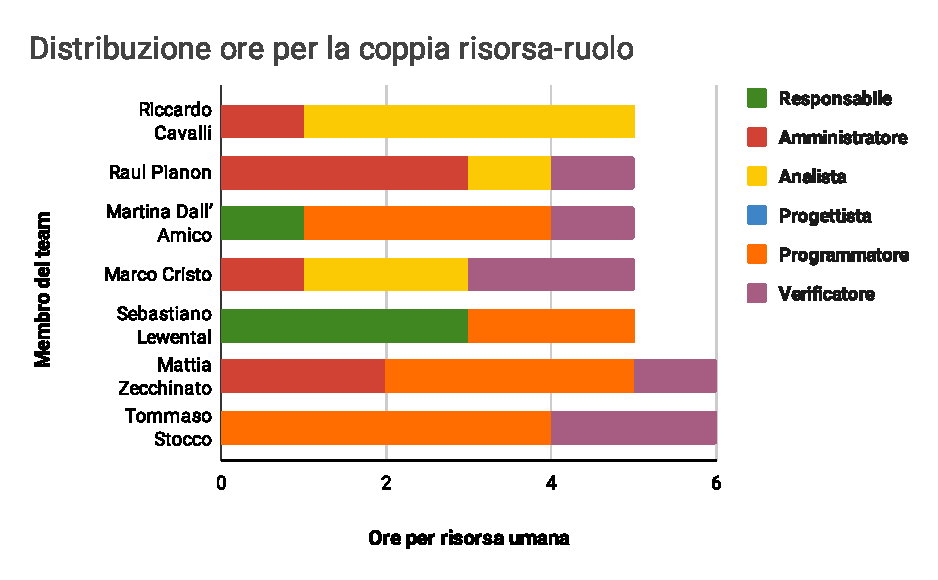
\includegraphics[width=0.90\textwidth]{assets/Consuntivo/Sprint-6/distribuzione_ore_risorsa_ruolo.pdf}
    \caption{Sprint 6 - Istogramma della distribuzione oraria per la coppia risorsa-ruolo}
  \end{figure}
  
  \begin{figure}[H]
    \centering
    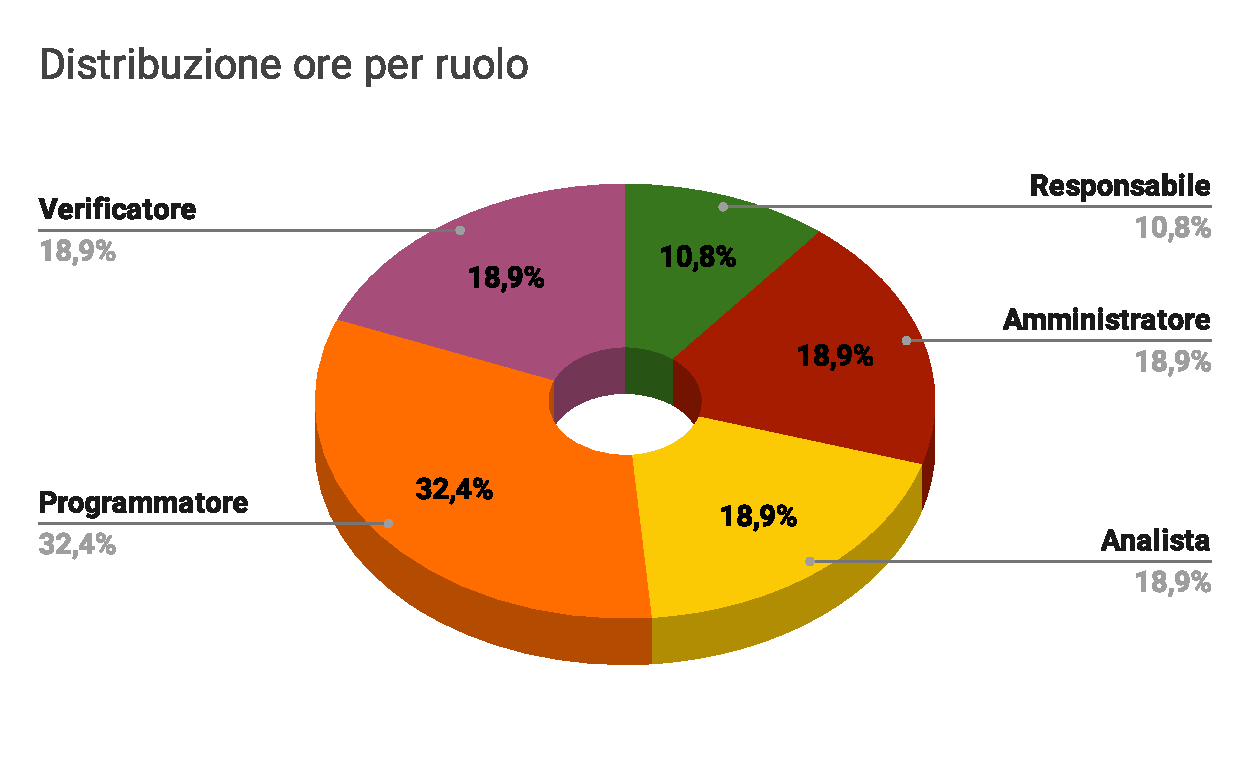
\includegraphics[width=0.90\textwidth]{assets/Consuntivo/Sprint-6/distribuzione_ore_ruolo.pdf}
    \caption{Sprint 6 - Areogramma della distribuzione oraria per ruolo}
  \end{figure}
  
  \begin{minipage}{\textwidth}
  Di seguito è riportato il consuntivo economico del sesto \glossario{sprint}:
  \begin{table}[H]
  \begin{adjustwidth}{-0.5cm}{-0.5cm}
    \centering
    \begin{tabular}{|P{2.9cm}|P{2.3cm}|P{2.5cm}|P{2.3cm}|>{\arraybackslash}P{2.5cm}|}
      \hline
      \multicolumn{5}{|c|}{\textbf{Consuntivo economico}} \\
      \hline
      \textbf{Ruolo} & \textbf{Ore per ruolo} & \textbf{Delta ore preventivo - consuntivo} & \textbf{Costo (in \texteuro)} & \textbf{Delta costo preventivo - consuntivo (in \texteuro)} \\
      \hline
      Responsabile & 4 & -1 & 120,00 & -30,00 \\ \hline
      Amministratore & 7 & 1 & 140,00 & 20,00 \\ \hline
      Analista & 5 & 1 & 125,00 & 25,00 \\ \hline
      Progettista & 0 & 0 & 0,00 & 0,00 \\ \hline
      Programmatore & 8 & 1 & 120,00 & 15,00 \\ \hline
      Verificatore & 4 & 0 & 60,00 & 0,00 \\ \hline
      \textbf{Totale} & \textbf{28} & 2 & \textbf{565,00} & 30,00 \\ \hline
      \textbf{Restante} & 380 & / & 7.515,00 & / \\ \hline
      \textbf{Sprint pregressi} & 236 & / & 4.905,00 & / \\ \hline
    \end{tabular}
    \caption{Sprint 6 - Consuntivo economico}
  \end{adjustwidth}
  \end{table}
  \end{minipage}
  
  \begin{figure}[H]
    \centering
    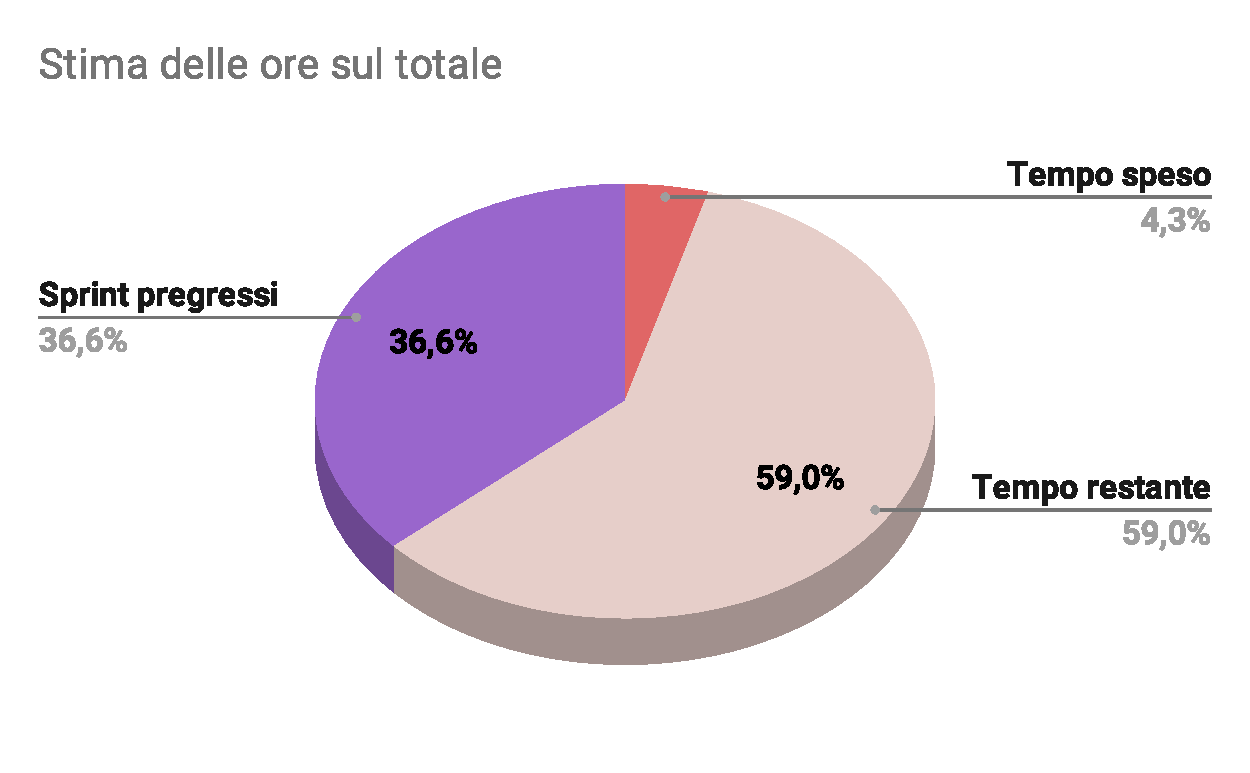
\includegraphics[width=0.90\textwidth]{assets/Consuntivo/Sprint-6/copertura_oraria.pdf}
    \caption{Sprint 6 - Areogramma del tempo speso (in ore) rispetto al totale}
  \end{figure}
  
  \begin{figure}[H]
    \centering
    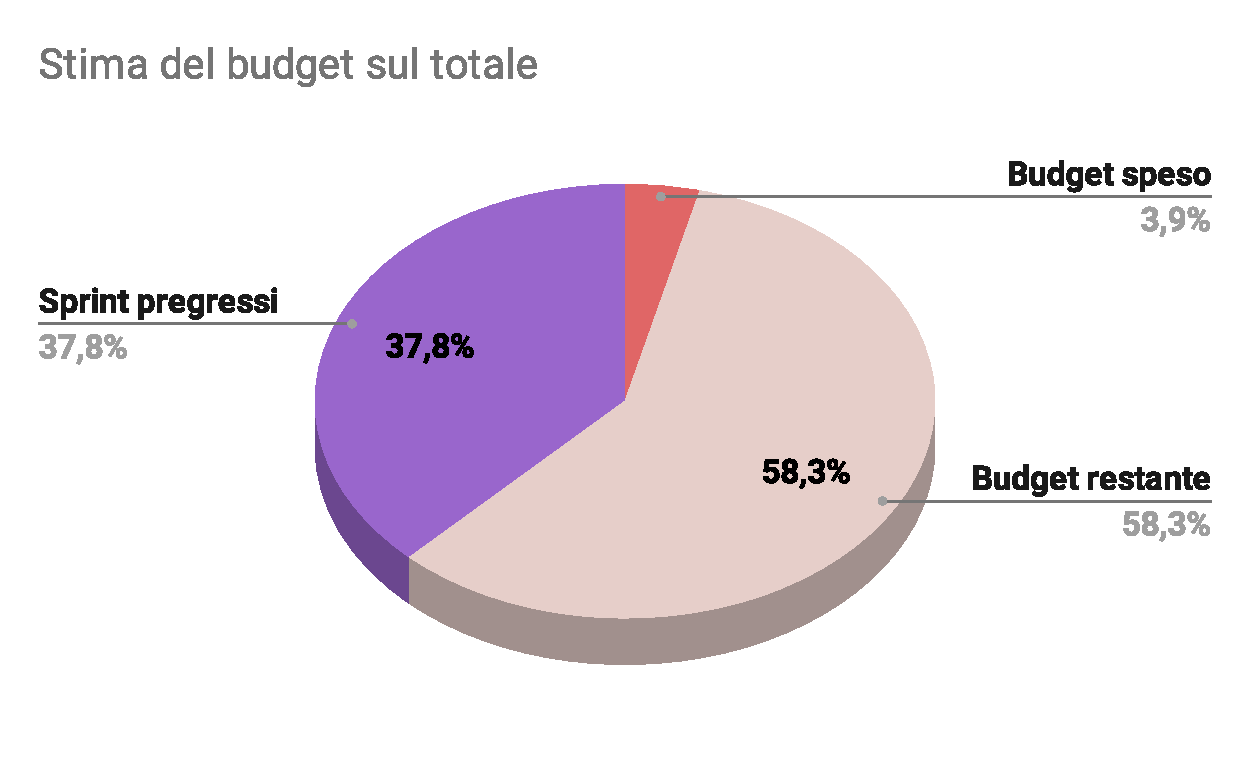
\includegraphics[width=0.90\textwidth]{assets/Consuntivo/Sprint-6/budget_speso.pdf}
    \caption{Sprint 6 - Areogramma del budget speso rispetto al totale}
  \end{figure}
  
  \begin{minipage}{\textwidth}
    Di seguito sono riportate le ore rimanenti per la coppia risorsa-ruolo:
    \begin{table}[H]
      \begin{tabularx}{\textwidth}{|c|*{6}{>{\centering}X|}c|}
        \hline
        \multicolumn{8}{|c|}{\textbf{Ore rimanenti per la coppia risorsa-ruolo}} \\
        \hline
        \textbf{Membro del team} & \textbf{Re} & \textbf{Am} & \textbf{An} & \textbf{Pt} & \textbf{Pr} & \textbf{Ve} & \textbf{Totale per persona} \\
        \hline
        Cavalli Riccardo & 0 & 0 & 4 & 14 & 16 & 15 & 49 \\ 
        \hline
        Pianon Raul & 2 & 7 & 1 & 20 & 10 & 12 & 52 \\ 
        \hline
        Dall’Amico Martina & 5 & 2 & 1 & 14 & 19 & 12 & 53 \\ 
        \hline
        Cristo Marco & 2 & 9 & 1 & 17 & 10 & 14 & 53 \\ 
        \hline
        Lewental Sebastiano & 6 & 4 & 2 & 11 & 17 & 15 & 55 \\ 
        \hline
        Zecchinato Mattia & 9 & 6 & 3 & 11 & 14 & 14 & 57 \\ 
        \hline
        Stocco Tommaso & 5 & 4 & 3 & 20 & 11 & 18 & 61 \\ 
        \hline
        \textbf{Totale ore per ruolo} & 29 & 32 & 15 & 107 & 97 & 100 & \textbf{380} \\ 
        \hline
      \end{tabularx}
      \caption{Sprint 6 - Ore rimanenti per la coppia risorsa-ruolo}
    \end{table}
  \end{minipage}

\subsubsection{Revisione delle attività}

Nell'arco del sesto \glossario{sprint}, il team ha svolto le seguenti attività:
\begin{itemize}
    \item Stesura dei verbali interni ed esterni;
    \item Miglioramento della struttura dei \glossario{casi d'uso} nell’\AdR;
    \item Revisione dei grafici nell’\AdR;
    \item Ampliamento dei casi d’uso con la gestione del \glossario{debug} e degli errori;
    \item Aggiornamento del \PdP; (stesura delle sezioni incomplete e revi-sione dei consuntivi precedenti);
    \item Stesura della dashboard di valutazione della qualità nel Piano di Qualifica;
    \item Inserimento dei grafici nel Piano di Qualifica;
    \item Creazione componente di login funzionante;
    \item Sviluppo delle pagine \glossario{front-end} (chat, gestione dei \glossario{dizionari dati} e debug).
\end{itemize}

\subsubsection{Retrospettiva}

\par Di seguito sono riportati i risultati del questionario di valutazione dello \glossario{sprint}:
\begin{itemize}
  \item Organizzazione dello \glossario{sprint}\ - Valutazione: 8;
  \item Conduzione dei meeting interni - Valutazione: 8;
  \item Conduzione dei meeting esterni - Valutazione: 8;
  \item Impegno e partecipazione dei singoli membri - Valutazione: 7;
  \item La quasi totalità dei membri del team era a conoscenza delle proprie mansioni;
  \item La numerosità delle riunioni è risultata adeguata per tutti i membri del gruppo;
  \item Le riunioni sono state organizzate quasi sempre con il giusto preavviso;
  \item Il rapporto ore spese/ore produttive si sta notevolmente equilibrando;
  \item La produttività è stata ragioneole considerando le criticità dell'imminente sessione;
  \item È diffusa l'idea di programmare incontri in presenza più frequenti.
\end{itemize}

\vspace{0.5\baselineskip}
\par A seguire le \textbf{analisi a posteriori} del sesto \glossario{sprint}:
\begin{itemize}
  \item In seguito ad un incontro in presenza avvenuto durante questo \glossario{sprint}, il team ha notato quanto più efficace risulti questa modalità di lavoro rispetto a quella a distanza, evidenziata dalla quantità di \glossario{pull request} avvenute e risolte in tale occasione;
  \item La sessione di esami ha impattato sulla quantità di lavoro svolto, come previsto.
\end{itemize}

\subsubsection{Aggiornamento pianificazione e preventivo}
\par Il team ha definito un piano d'azione per migliorare l'organizzazione e la produttività del prossimo \glossario{sprint}:
\begin{itemize}
  \item Pianificare incontri in presenza con frequenza maggiore, di almeno un incontro ogni due settimane;
\end{itemize}

\paragraph*{Pianificazione futura:}
\par Come riportato nell'analisi a posteriori, il team ha deciso di aumentare il numero di riunioni in presenza.
Inoltre si è deciso di mantenere moderata la quantità di ore assegnate a ciascun membro del team, in modo da continuare a garantire un equilibrio tra lavoro e studio.

\paragraph*{Preventivo "a finire" (\sezione{sec:stima_temporale}):}
\par L'avanzamento dello stato prodotto porta a stabilire la prossimità della revisione RTB, che avverrà tuttavia dopo la sessione di esami.

\paragraph*{Gestione dei rischi (\sezione{sec:analisi_rischi}):}
\par Nel corso del sesto \glossario{sprint}, alcune contromisure si sono rivelate insufficienti a mitigare i rischi emersi:
\begin{itemize}
  \item \textbf{RO4 - Rotazione dei ruoli}: nonostante il team avesse previsto di affiancare alcuni membri esperti ai nuovi programmatori, la concomitanza degli esami ha impedito l'attuazione di questa misura di mitigazione. Il rischio è stato gestito attraverso l’organizzazione di un incontro in presenza, durante il quale il gruppo ha completato le attività con la priorità più alta. Nella \sezione{sec:analisi_rischi}, il rischio relativo alla rotazione dei ruoli è stato aggiornato, con gli incontri in presenza considerati come possibili contromisure.
\end{itemize}

\par Di seguito sono elencati i rischi gestiti con successo:
\begin{itemize}
  \item \textbf{RO1 - Periodi di rallentamento}: in prossimità della sessione di esami, il team ha avuto difficoltà a conciliare l'avanzamento del progetto e lo studio personale; pertanto, le ore produttive individuali sono state ridotte. Trattandosi di un rischio preventivato, il gruppo è riuscito a mantenere un flusso di lavoro regolare;
  \item \textbf{RT3 - Malfunzionamenti software}: le anomalie software sono state trattate nel canale dedicato su Discord e risolte attraverso l'apertura di issue su GitHub.
  \item \textbf{RT1 - Scarso know-how tecnologico}: attraverso il processo di integrazione continua, il team ha potuto allinearsi con le soluzioni sviluppate nello sprint precedente.
\end{itemize}
